In this chapter, I will present the two phases learning process utilized by a fully connected neural network (FCNet) to maximize the agents' utility. During phase 1, the agents' objective will be to maximise utility when labour is gradually introduced. While in phase 2, there will be the introduction of a tax. In this chapter, I will present four taxation mechanisms, two of which are the same as the paper of reference, while the others are an extension of mine. In conclusion, I will present the results derived from the training and a discussion on the values obtained.

\section{Experiment Setup}

After understanding the Foundation framework and the process used by RL to optimize a policy, we can focus on the model used. In the reference paper, the authors used a combination of a convolutional neural network and an LSTM \cite{zheng2020ai}. This could grant them good spatial information from the CNN and memory cells from the LSTM. These features are appropriate because there is the need of processing a map and the agents share the same network.

In the experiments, however, it was used a fully connected neural network that does not share the same features as the one above. The complete structure of the model is shown in Table \ref{tab:Fcnet}. 


\begin{table}[h!]
    \begin{tabular}{llll}
	Model: "FCNet"            &                    &          &                            \\ \hline
	Layer (type)              & Output Shape       & Param \# & Connected to               \\ \hline
	observations (InputLayer) & {[}(None, 1260){]} & 0        &                            \\ \hline
	encoder (Encoder)         & (None, 256)        & 389632   & observations{[}0{]}{[}0{]} \\ \hline
	fc\_out (Dense)           & (None, 50)         & 12850    & encoder{[}0{]}{[}0{]}      \\ \hline
	value\_out (Dense)        & (None, 1)          & 257      & encoder{[}0{]}{[}0{]}      \\ \hline
	Total params: 402,739     &                    &          &                            \\
	Trainable params: 402,739 &                    &          &                            \\
	Non-trainable params: 0   &                    &          &                            \\ \hline
    \end{tabular}
    \caption{\label{tab:Fcnet} Fully connected neural network utilized.}
\end{table}

This setup might incur a loss of efficiency for plenty of reasons. First of all, as said before, the features of the LSTM/CNN are missing. Following, due to lack of resources, it was not possible to do a proper hyperparameter tuning. However, as we will see, the FCNet can provide us with meaningful results, in particular, the agents will show emerging behaviours and specialization. These are characteristics that were also found in the paper by Zheng and Trott, the difference stands in the agents' efficiency which is lower for the model used here.

There are many parameters that have to be set at this stage (for a semi-complete list check the Appendix Table \ref{tab:hyperparameter_env} and Table \ref{tab:hyperparameter_train}). The first part of such values is related to the training, while the second part is to the environment. I would like to stress some of the latter parameters, to better understand the simulation.

First, the skill levels are set to be different for each agent. The skill is the number of coins received when building a house. The four skills are fixed and they are taken from a Pareto Distribution. Namely the values are (11.3; 13.3; 16.5; 22.2). These values are always assigned to the same starting location in the map, thus the agent starting in the bottom right will always have the highest skill, and so on. Other important parameters are the episode length \( H \) which is set to 1000 time steps, the resource re-spawn probability which is set to 1\% per time step, and the initial coin endowment that is set to 0.

Once the environment is defined, it is possible to start the training which will occur in two phases. The first phase introduces labour, while the second introduces taxation.

\section{Phase 1 training}

The first training phase is necessary to get the FCNet in Table \ref{tab:Fcnet} accustomed to the world dynamics and avoid falling into un-optimal behaviour once disincentives factors are introduced. These two factors, as already discussed, are labour costs and taxation. At this moment, I am interested in getting the agent accustomed to the labour costs, while the taxes are completely removed and will be addressed in the second phase of the training. 


\begin{figure}[h!]
    \centering
    \linespread{.9} 
    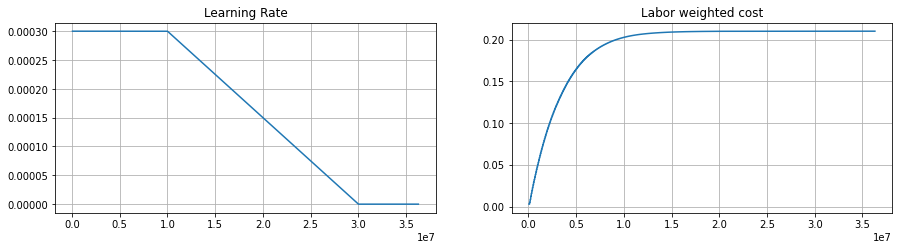
\includegraphics[width=0.95\textwidth]{Resources/imgs/LR_phase1.png}
    \caption[Learning rate and Labor weighed cost for Phase 1 training: ]%
    {\label{img:lr_phase0}Learning rate and Labor weighed cost for Phase 1 training: \small \textit{this was the schedule for respectively the learning rate and the labor cost in the phase 1 of the training, here the learning rate goes to 0 because we don't seek convergence now.}}
\end{figure}

The training agenda is built to run for a total of 30M time-steps, as we can see from Figure \ref{img:lr_phase0} the learning rate is set to be at 3e-4 for 10M steps, then it linearly reduces to 0 in 20M time-steps. Meanwhile, the labour weight increases following the function:

\begin{equation}
    \vartheta_k = 1- exp\left(- \frac{\textit{number of time mean reward }> 0}{\textit{energy warm-up constant (k)}}\right)
\end{equation}

where the warm-up constant is set to 10000. This setup gives the FCNet time to learn how to respond properly to the dis-utility generated by the labour. 



\begin{figure}[h!]
    \centering
    \linespread{.9} 
    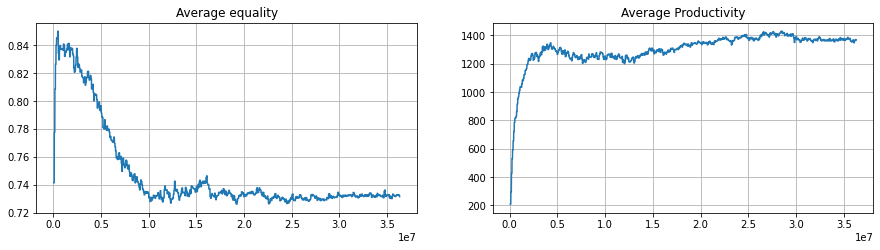
\includegraphics[width=0.95\textwidth]{Resources/imgs/FCNET_prod_phase1.png}
    \caption[Equality and Productivity during Phase 1:  ]%
    {\label{img:prod_phase0}Equality and Productivity during Phase 1: \small \textit{here we have the evolution of equality between agents and total production in the training of phase 1}}
\end{figure}


In Figure \ref{img:prod_phase0}, we can observe two of the most important variables we are considering: equality and productivity. On the left, we have the average equality, calculated by the following formula:

\begin{equation}
    equality(\mathbf{x^c_{t}}) = 1 - \frac{N}{N-1} \frac{\sum^N_{i=1}\sum^N_{j=1}| x^c_{i,t} - x^c_{j,t}|}{2N\sum^N_{i=1}x^c_{i,t}}
\end{equation}

with \( 0 < equality(\mathbf{x^c_{t}}) < 1 \). This function returns 1 if the endowments are equally split between the N (4) agents, and 0 if one agent owns all of the coins in the economy. What we observe is that after 36M time-steps the equality settles around 0.73, this is justified by the difference in coin endowment between the agent with the highest skill (Agent 0 in Figure \ref{img:p0_brakedown}) and the other agents. Furthermore, we can notice that the average productivity of the economy settles around 1400. However, both of these values are incorrect because of a data collection issue in the code. We will discuss later the actual values.


\begin{figure}[h!]
    \centering
    \linespread{.9}
    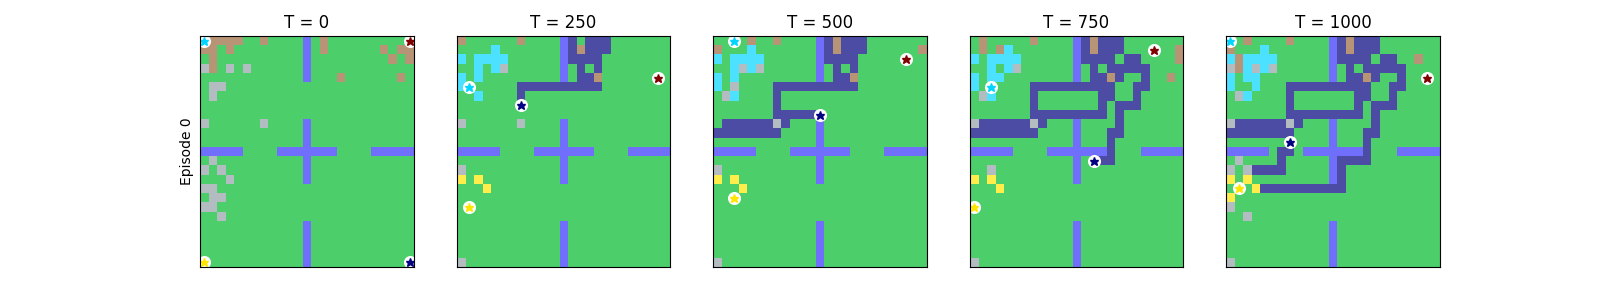
\includegraphics[width=0.95\textwidth]{Resources/imgs/Figure_1.png}
    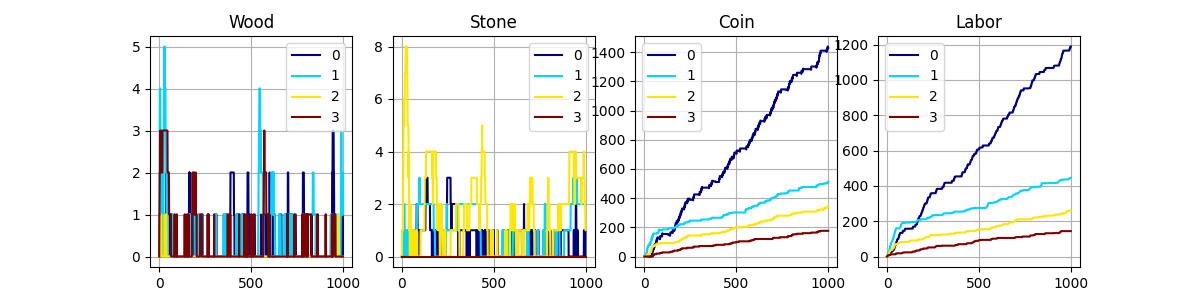
\includegraphics[width=0.80\textwidth]{Resources/imgs/Figure_2.png}
    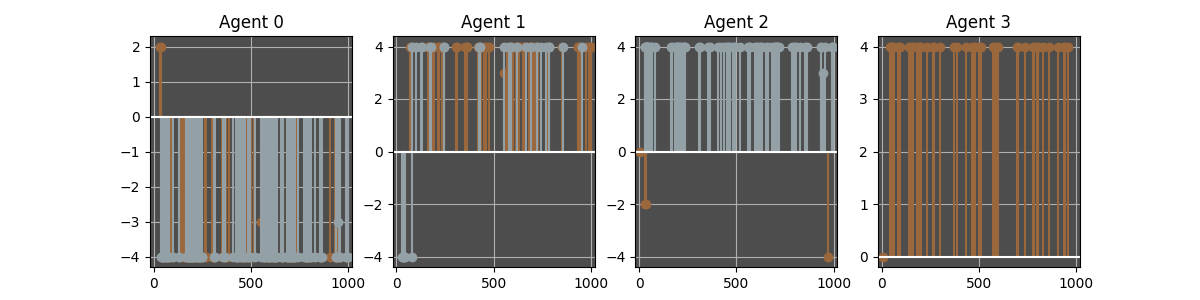
\includegraphics[width=0.80\textwidth]{Resources/imgs/Figure_3.png}
    \caption[Phase 1 full brake down: ]%
    {\label{img:p0_brakedown}Phase 1 full brake down: \small \textit{this is a more complete overview of one random simulation crated using the weights at the end of phase 1 training}}
\end{figure}

Regardless, the results obtained so far are not important for the final analysis because there was no criterion used to stop the training and the learning rate was decreased to 0. This means that the FCNet might not have reached convergence nor an optimal policy. Nonetheless, we can keep these results in mind as a benchmark for the phase 2 training, as we will use the weights obtained to carry on the training.

In conclusion, the most important result from the first training is that agents show emerging behaviours. We can see that the agents specialize in a specific task according to their initial position on the map and their skill level. Behaviours are important to the scope of the thesis because it is hard to capture specialization analytically. Here, instead, it is rather easy to have specialized agents as their utility is maximized through experience.

From Figure \ref{img:p0_brakedown}, we can see that the agent with the highest skill has specialized in building houses, this makes sense since he earns more from the building action. By building he can also afford to buy goods from the market, giving other agents the possibility to specialize in gathering and selling. Indeed, this behaviour is adopted by agents 2 and 3, as they are those endowed with the lowest skills. On the other hand, agent 1 exhibits a variable behaviour. He sells goods in the market, given that he has both of them available in his macro-area, but at the same time he exerts some labour to build houses.

\section{Phase 2 Training}

  
In the second phase of the training, the learning rate schedule is changed to be 3e-4 for the first 35M time-steps and then will linearly decrease to 1e-6 in a span of 15M time-steps. This will grant a faster learning rate in the initial part of the training when the FCNet will suffer a huge decrease in efficiency due to the introduction of the taxation. 

The starting point for this second phase is the weights obtained from phase 1, and the training will be formed by four different simulations diverging from this initial state. These simulations are US taxation, Italian Taxation, free-market and Communism.

\subsection{Free Market}

Free-market is the first and simplest kind of simulation that we can carry out starting from the result in phase 1. This training consists in keep training the FCNet without imposing any kind of taxation. 

It is reasonable to believe that the result of this first training should generate a more productive economy. Or at least is what should be expected from economical theory \cite{atkinson2015lectures}. However, the equality between agents might suffer from higher production.

\subsection{US taxation}

The second kind of taxation used is US taxation. This is based on the 2018 Federal brackets and percentages. In particular we can see from Table \ref{tab:us_tax} the detailed structure. 


\begin{table}[h!]
\linespread{.9}
\begin{adjustbox}{max width=\textwidth}
    \begin{tabular}{llllllll}
        \hline
    Bracket in \$   & 0-9700 & 9700-39475 & 39475-84200 & 84200-160725 & 160725-204100 & 204100-510300 & 510300+ \\
    Bracket in Coin & 0-9.7  & 9.7-39.5   & 39.5-84.2   & 84.2-160.7   & 160.7-204.1   & 204.1-510.3   & 510.3+  \\
    Tax*            & 10\%   & 12\%       & 22\%        & 24\%         & 32\%          & 35\%          & 37\%\\
    \hline
    \end{tabular}
\end{adjustbox}
    \caption[2018 US federal tax system:]%
    {\label{tab:us_tax}2018 US federal tax system: \small \textit{this is the proportional system that was in place in the US in 2018, notice that the tax is marginal (i.e. if you are in the second bracket you will pay 970\$ + 12\% of the amount above 9700\$) }}
\end{table}


With the introduction of these lump-sum tax plus redistribution is easy to conclude that there might be an increase in equality, however, this might produce a negative effect on total production since the high-skilled agent are disincentivised to produce.

\subsection{Italian Taxation}

Like the US system, the Italian one is a marginal system with brackets, however in this case the fiscal pressure is higher and the brackets smaller. As a reference, it was used the 2020 INPS brackets and percentages (Table \ref{tab:ita_tax}). However, the brackets were calculated in dollars, so all the values were multiplied by 1.1575, the exchange rate at October 1st 2021.



\begin{table}[h!]
\linespread{.9}
    \begin{adjustbox}{max width=\textwidth}
        \begin{tabular}{llllll}
            \hline
        Bracket in \EURcr   & 0-15000 & 15000-28000 & 28000-55000 & 55000-75000 & 75000+ \\
        Bracket in Coin & 0-17  & 17-32  & 32-63  & 63-86   &  86+   \\
        Tax*            & 23\%   & 27\%       & 38\%        & 41\%         & 43\%       \\
        \hline
        \end{tabular}
    \end{adjustbox}
        \caption[2020 INPS tax system:]%
        {\label{tab:ita_tax}2020 INPS tax system: \small \textit{this is the proportional system that was in place in the Italy in 2020, notice that the tax is marginal (i.e. if you are in the second bracket you will pay 3450\EURcr + 27\% of the amount above 15000\EURcr) }}
    \end{table}



In this case, there is an even higher pressure, which might push toward higher equality and lower total production.


\subsection{Communism}


Communism is the opposite of the Free market, in this simulation the fiscal pressure is 1, meaning that every 100 time-step all the agents are taxed for the entire amount of coins they own and then redistributed. This system will probably deliver the lowest production and the highest equality.


\section{Training Results}

The process of training is computationally complex. It requires a good machine and plenty of time. In this case, there were used multiple machines and the trial period on Microsoft Azure allowed the use of up to 4 CPUs. No GPUs were implemented for the training purpose since it wasn't present in all the machines. However, by implementing an FCNet instead of a CNN the loss of efficiency the lack of GPU is not enormous.

The time needed to run a single training for 200M of time-steps was between 100/200h depending on the machine. This huge amount of time needed did not give any possibility to do hyper-parameter training of any sort to increase efficiency, nor to check the consistency of the results.

\begin{figure}[h!]
    \centering
    \linespread{.9}
    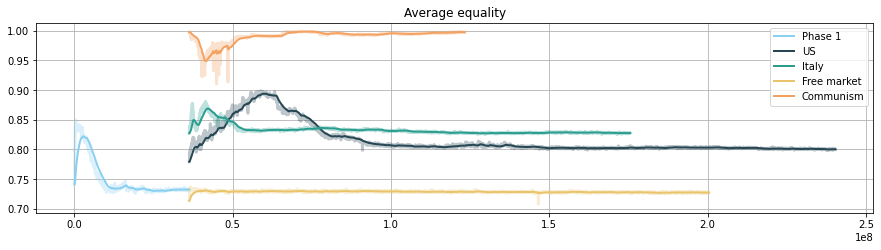
\includegraphics[width=0.95\textwidth]{Resources/imgs/equality_training.png}
    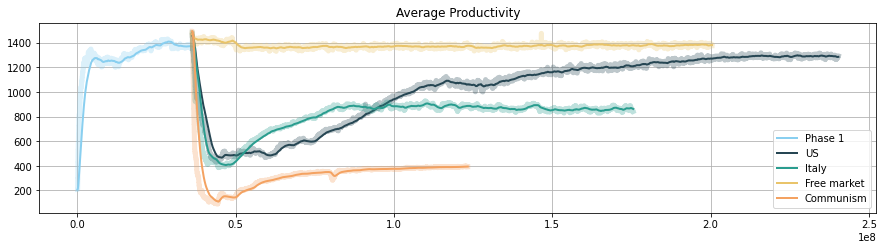
\includegraphics[width=0.95\textwidth]{Resources/imgs/productivity_training.png}
    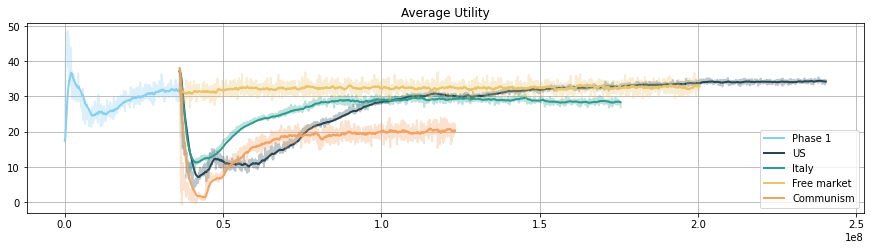
\includegraphics[width=0.95\textwidth]{Resources/imgs/utility_training.png}
    \caption[Phase 2 training brake down: ]%
    {\label{img:p1_brakedown}Phase 2 training brake down: \small \textit{here we can see the training process, on the horizontal axis there are the time-steps, the training lasted for around 200M steps per simulation, and in the graphs is possible to see the evolution of equality, productivity and utility of the agents on average.}}
\end{figure}


In Figure \ref{img:p1_brakedown} we can see the full training process for these simulations. We could start to draw some conclusions from it, however, the values displayed are not representative of the true production and equality. We can see it in Figure \ref{img:prod_phase0} where the average production is around 1400, whereas in Figure \ref{img:p0_brakedown} the total actual production is above 2500. This is not just a right tale coincidence. This is an issue (in data collection) that I discovered once all the data was trained, thus it is impossible to recreate the correct graphs unless running all the training again (800+ hours).

To produce valid and comparable results, the weights obtained from the training were used to run 1000 simulations. With this data set, now is possible to generate reliable and comparable data.



\begin{figure}[h!]
    \centering
    \linespread{.9}
    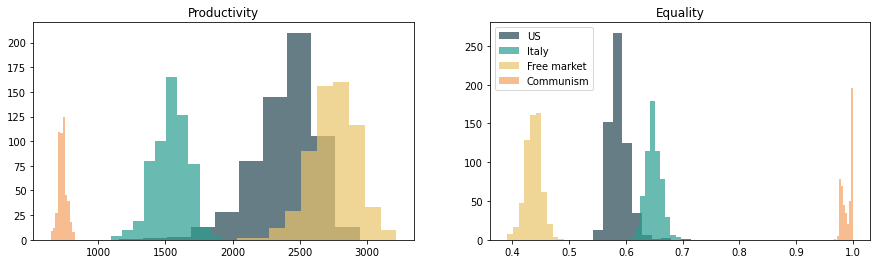
\includegraphics[width=0.95\textwidth]{Resources/imgs/hist.png}
    \caption[Productivity and Equality histogram: ]%
    {\label{img:hists}Productivity and Equality histogram: \small \textit{these are the two histograms with the correct data on production (on the left) and equality (on the right). The color coding is the same across the two graphs.}}
\end{figure}


The first comparisons that are presented are the histograms on Figure \ref{img:hists}. In particular we have that the most productive economy is the Free market with an average production of 2751 (\(\sigma = 161\)), and at the same time is the one with the highest disparity, 0.437 (\(\sigma = 0.014\)). US economy is the second most productive
2393 (\(\sigma = 235\)) and with equality 0.587 (\(\sigma = 0.017\)). Italy has a production of 1548 (\(\sigma = 125\)) and agents have a coin equality of 0.64 (\(\sigma = 0.013\)). And finally the Communism has the highest level of equality 0.99 (\(\sigma = 0.009\)) and the lowest total productivity 732 (\(\sigma = 32\)).

If we compare the results obtained so far with the one in the paper of Zheng and Trott, we can see that there is a loss in efficiency of -16.3\% in Free market productivity and of 12\% in equality. For the US instead, -10\% and 22\% respectively. This loss in overall efficiency was already expected as discussed above.

\begin{figure}[h!]
    \centering
    \linespread{.9}
    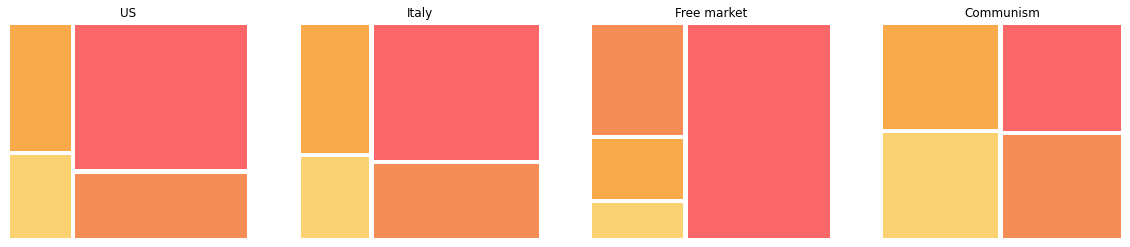
\includegraphics[width=0.75\textwidth]{Resources/imgs/coin_distr.png}
    \caption[Coin Distribution]%
    {\label{img:coin_distribution}Coin Distribution: \small \textit{this is a graphical representation of the coin distribution in the 4 experiments. The darker the color the richer the agent. The areas are proportional to the amount of economy owned by the agent.}}
\end{figure}

To have a better understanding of these results, we can check Figure \ref{img:scatter}. In this figure, equality is plotted in the plane against productivity. If we take into consideration the two systems that are actually used (US and Italy), we can see how the fiscal pressure given by Italian brackets and percentages causes a loss in productivity of about 35.4\% compared to the US, but there is a gain of only 10.54\% in equality.

\begin{figure}[h!]
    \centering
    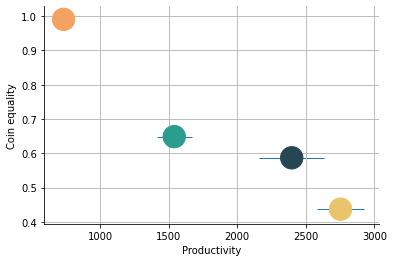
\includegraphics[width=0.45\textwidth]{Resources/imgs/scatter.png}
    \caption[Coin Distribution]%
    {\label{img:scatter}Coin Distribution \small \textit{}}
\end{figure}


The last performance measure that could be taken into consideration is the product of the previous two. It makes sense, as a policymaker, to try to maximize not only the production or the equality but both of them at the same time as seen in economical theory \cite{saez2001using}. Thus the usage of the product of the two measures seen so far could be a good candidate objective for the tax maker. in Figure \ref{img:eqxprod_hist} we can see the distribution of this value across the 4 experiments. Here is noticeable how the US economy shows a higher value compared to the Free market. 

\begin{figure}[h!]
    \centering
    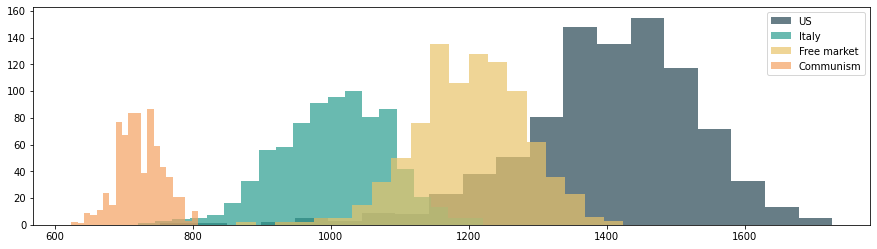
\includegraphics[width=0.95\textwidth]{Resources/imgs/coin_times_eq.png}
    \caption[Coin equality times total production]%
    {\label{img:eqxprod_hist}Coin equality times total production\small \textit{}}
\end{figure}



These results, however, are not representative of the real impact of the actual taxation systems on the population. This simulation is still far away from reality. In addition, several necessary tests on consistency of the results and hyperparameter tuning are missing. 

However, we can still conclude that AI-driven agents can perform tasks that otherwise would be impossible to model. The economical relevance of the results is now questionable, however, it could be interesting to further develop simulations where economical agents are subject to RL optimization. The use of such simulations could be a starting point to check whether the agents' behaviour converges to the analytical behaviour. Moreover, my work can be developed into more complex simulations to explore the effect of policies.